\documentclass{article}[12pt]

\usepackage[utf8]{inputenc}
\usepackage{amsfonts,amssymb,amsmath,subfigure}
\usepackage[pdftex]{graphicx}
\usepackage{epstopdf}
\usepackage{vmargin}
\usepackage{comment}
\usepackage{tikz,multicol}

\usepackage{algorithm}
\usepackage[noend]{algpseudocode}
\usepackage{tcolorbox}

\newtcolorbox{mybox}[3][]
{
  colframe = #2!25,
  colback  = #2!10,
  coltitle = #2!20!black,  
  title    = {#3},
  #1,
}


\newcommand*\Let[2]{\State #1 $\gets$ #2}
\algrenewcommand\algorithmicrequire{\textbf{Precondition:}}
\algrenewcommand\algorithmicensure{\textbf{Postcondition:}}




\excludecomment{solution}
%\includecomment{solution}

\title{IF111 - Algorithmes et structures de données\\EI6 - Examen Blanc}
\date{\texttt{rfosse@labri.fr}}
\author{Rohan Fossé}
\begin{document}



\maketitle{}

\section{Multiplication Russe}
On considère l’algorithme suivant qui calcule et retourne la multiplication de deux entiers positifs $m$ et $n$ :

\begin{tcolorbox}
        \begin{algorithmic}[1]
    \Function{$mult$}{$m,n$}
    \Let{$r$}{$0$}
    \While{\text{$n > 0$}}
        \If{\text{$n \% 2 == 1$}}
            \Let{$r$}{$r + m$}
        \EndIf
        \Let{$m$}{$m * 2$}
        \Let{$n$}{$n // 2$}
    \EndWhile
    \State\text{\textbf{return r}}
  \EndFunction
  \end{algorithmic}
 \end{tcolorbox} 

\begin{enumerate}
    \item Compter le nombre d’opérations primitives exécutées à chaque ligne.
    \item En majorant ce nombre, donner une complexité en temps dans le pire cas par rapport à n.
\end{enumerate}


\section{Fonction d'Ackermann}
Ecrire un algorithme récursif qui calcule $A(m, n)$ définit comme ceci:

$$
\left\{
    \begin{array}{ll}
        A(0,n) = n + 1 \\
        A(m,0) = A(m - 1, 1), \text{pour m} > \text{0}\\
        A(m,n) = A(m - 1,A(m,n - 1)), \text{pour m} > \text{0 et n} > \text{0}
    \end{array}
\right.
$$

\begin{figure}
    \centering
    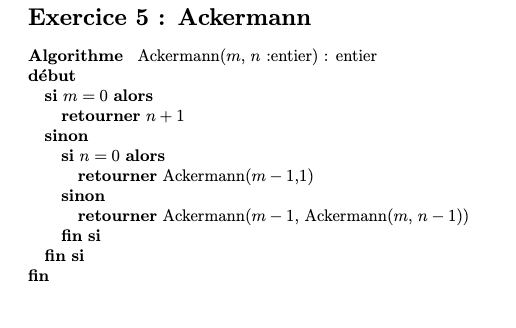
\includegraphics[scale=0.4]{Ackerman.png}
    \label{fig:my_label}
\end{figure}

\section{Recherche dichotomique}
Écrire un algorithme récursif de recherche dichotomique d'un élément dans un tableau ordonné.

Dans les deux exercices suivants, vous pourrez utiliser les fonctions suivantes : 
\begin{itemize}
    \item $vide(l)$ : Renvoie $True$ si la liste $l$ est vide et $False$ sinon;
    \item $cons(a,l)$: Renvoie la liste obtenue en ajoutant l'élément $a$ devant la liste $l$;
    \item $tete(l)$: Renvoie le premier élément de la liste $l$;
    \item $queue(l)$ Renvoie la queue de la liste, ie $l$ sans le premier élément.
\end{itemize}

\begin{figure}[h!]
    \centering
    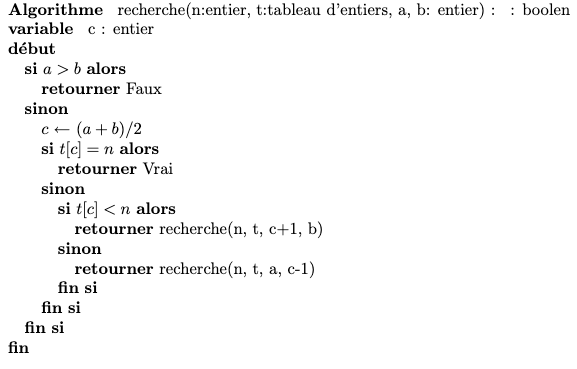
\includegraphics[scale=0.4]{Dic.png}
    \label{fig:my_label}
\end{figure}

\section{Nombre d'occurrence}
Définir un algorithme qui compte le nombre d'occurrence d'un élément $x$ dans une liste donnée.

\begin{figure}[h!]
    \centering
    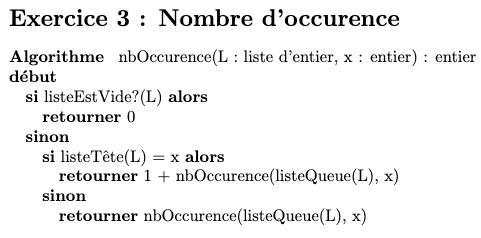
\includegraphics[scale=0.4]{Occ.png}
    \label{fig:my_label}
\end{figure}

\section{Retournement}
Définir un algorithme qui inverse l'ordre des éléments d'une liste $l$.

\begin{figure}[h!]
    \centering
    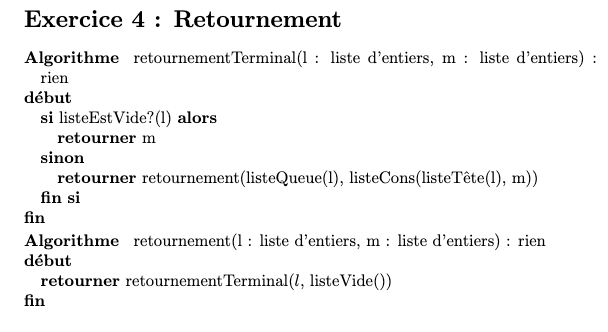
\includegraphics[scale=0.4]{Retournement.png}
    \label{fig:my_label}
\end{figure}


\section{Tas min}
Écrire une fonction qui vérifie si un arbre binaire est un tas min. Quelle est sa complexité ?


\section{Le robot}
Un robot se promène sur le graphe \ref{fig:robot}. Partant d’un sommet quelconque s, appelé sommet de stockage, il doit déposer un cube sur chacun des autres sommets. Il possède suffisamment de cubes sur le sommet de stockage, mais ne peut transporter qu'un cube à la fois (il doit donc repasser par le sommet de stockage avant de livrer un autre cube).
\begin{enumerate}
    \item Calculer, pour chacun des sommets du graphe, le trajet minimum que doit parcourir le robot si ce sommet est sommet de stockage.
    \item Quel est le "meilleur" sommet de stockage ?
\end{enumerate}

\begin{figure}[h!]
    \centering
    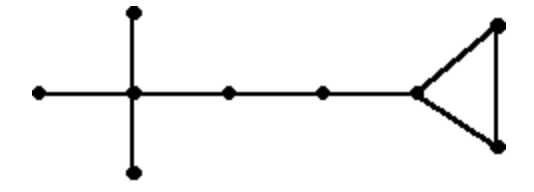
\includegraphics{Robot.png}
    \caption{Graphe du robot}
    \label{fig:robot}
\end{figure}

\section{Le facteur}
 Le graphe ci-dessous représente le plan d'une agglomération. Les sommets B, C, D, E, F et G désignent des villes. Une arête représente le trajet entre deux villes et est pondérée par le nombre de feux tricolores situés sur ce trajet. \\

\begin{figure}[h!]
    \centering
    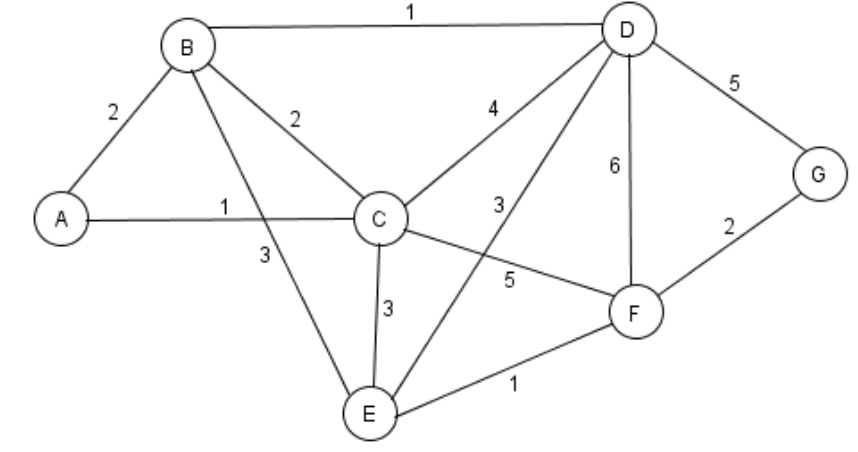
\includegraphics[scale=0.6]{Djisktra.png}
    \label{fig:my_label}
\end{figure}

 On s'intéresse au graphe non pondéré. Répondre aux questions suivantes :
\begin{enumerate}
    \item Ce graphe est-il connexe ?
    \item Ce graphe est-il complet ?
    \item Ce graphe admet-il une chaîne eulérienne ?
    \item Ce graphe admet-il un cycle eulérien ?
    \item Déterminer, en justifiant, le nombre chromatique de ce graphe.
\end{enumerate}
On s'intéresse dorénavant au graphe pondéré. Proposer un trajet comportant un minimum de feux tricolores reliant A à G.



\end{document}